\section{Forbedret navigasjon}
\label{sec:del3-navigasjon}

Denne delen beskriver navigasjonskomponentene i prototypen. Vi starter med
å kartlegge navigasjonen på helsedirektoratet.no slik den er i dag, og peker
på konkrete begrensninger. Deretter presenterer vi syv forbedringer vi har
implementert, med en før/etter-gjennomgang for hver. Motivasjonen for
valgene er forankret i funn fra brukerundersøkelsene (se
\autoref{sec:brukerundersokelser}).


\subsection{Sidehierarki og navigasjonsstruktur}
\label{sec:sidehierarki}

Nettsiden er strukturert i et hierarki med fire nivåer, fra forside til
individuelle innholdssider. Hierarkiet bestemmer hvordan breadcrumbsen
bygges opp, og gir brukeren en klar oversikt over hvor i nettstedet de
befinner seg.

\begin{figure}[H]
    \centering
    \includesvg[width=1.0\textwidth]{Images/Figures/sidehierarki}
    \caption{Sidehierarki -- navigasjonsstruktur fra forside til
             innholdssider, med eksempel på breadcrumbs.}
    \label{fig:sidehierarki}
\end{figure}

Hierarkiet er organisert som følger:

\begin{enumerate}
    \item \textbf{Forside} (\texttt{/}) -- inngangspunktet til nettstedet.
    \item \textbf{Temaside kategorier} -- syv overordnede temaer
          (f.eks.\ \textit{Forebygging, diagnose og behandling},
          \textit{Digitalisering og e-helse}) som hver representerer et
          faglig område.
    \item \textbf{Temaside} -- en spesifikk side innenfor en temakategori,
          identifisert av URL-stien \texttt{/:temaKategori/:temaNavn}.
    \item \textbf{Innholdssider} -- de faktiske innholdssidene brukeren
          navigerer til. Disse finnes i flere typer: nyheter
          (\texttt{/nyheter/...}), artikler, rapporter
          (\texttt{/statistikk/...}), retningslinjer
          (\texttt{/retningslinjer/...}) og statistikk.
\end{enumerate}

Breadcrumbsen reflekterer dette hierarkiet direkte, slik som vist i
eksempelet nederst i \autoref{fig:sidehierarki}:
\textit{Forside › Forebygging, diagnose og behandling › Diabetes ›
Nasjonal retningslinje for diabetes}.

% ─────────────────────────────────────────────────────────────
\subsection{Navigasjon på helsedirektoratet.no i dag}
\label{sec:nav-i-dag}


% TODO: Legg inn skjermbilde av dagens hd.no header/meny/brødsmulesti
% \begin{figure}[H]
%     \centering
%     \includegraphics[width=0.9\textwidth]{Images/Screenshots/hd-nav-idag}
%     \caption{Navigasjon på helsedirektoratet.no per 2025.}
%     \label{fig:hd-nav-idag}
% \end{figure}

Navigasjonsstrukturen på helsedirektoratet.no har i dag følgende
karakteristika:

\begin{itemize}
    \item \textbf{Breadcrumbs:} Sidene har breadcrumbs, men den er ikke
          konsekvent synlig på alle innholdstyper og gir begrenset
          kontekstuell støtte på dype sider.
    \item \textbf{Meny:} En global meny gir tilgang til de ulike
          fagområdene, men presentasjonen er flat og gir lite visuell
          støtte til å forstå hierarki og innholdets omfang.
    \item \textbf{Innholdssider:} Lange dokumenter (retningslinjer,
          veiledere) mangler en lokal innholdsfortegnelse i sidemeny.
          Brukeren må scrolle for å navigere i dokumentet.
    \item \textbf{Søkeintegrasjon i navigasjon:} Søket er separert fra
          navigasjonen, og resultatene gir lite kontekstuell filtrering
          etter innholdstype.
\end{itemize}

Funn fra brukerundersøkelsene (se \autoref{sec:brukerundersokelser})
understøtter at disse begrensningene skaper friksjon, særlig for
fagpersoner som navigerer i komplekse dokumentstrukturer.

% ─────────────────────────────────────────────────────────────

% ─────────────────────────────────────────────────────────────
\subsection{Breadcrumbs}
\label{sec:brodsmulesti}

\subsubsection{Dagens løsning}
\label{sec:brodsmulesti-idag}


\begin{figure}[H]
    \centering
    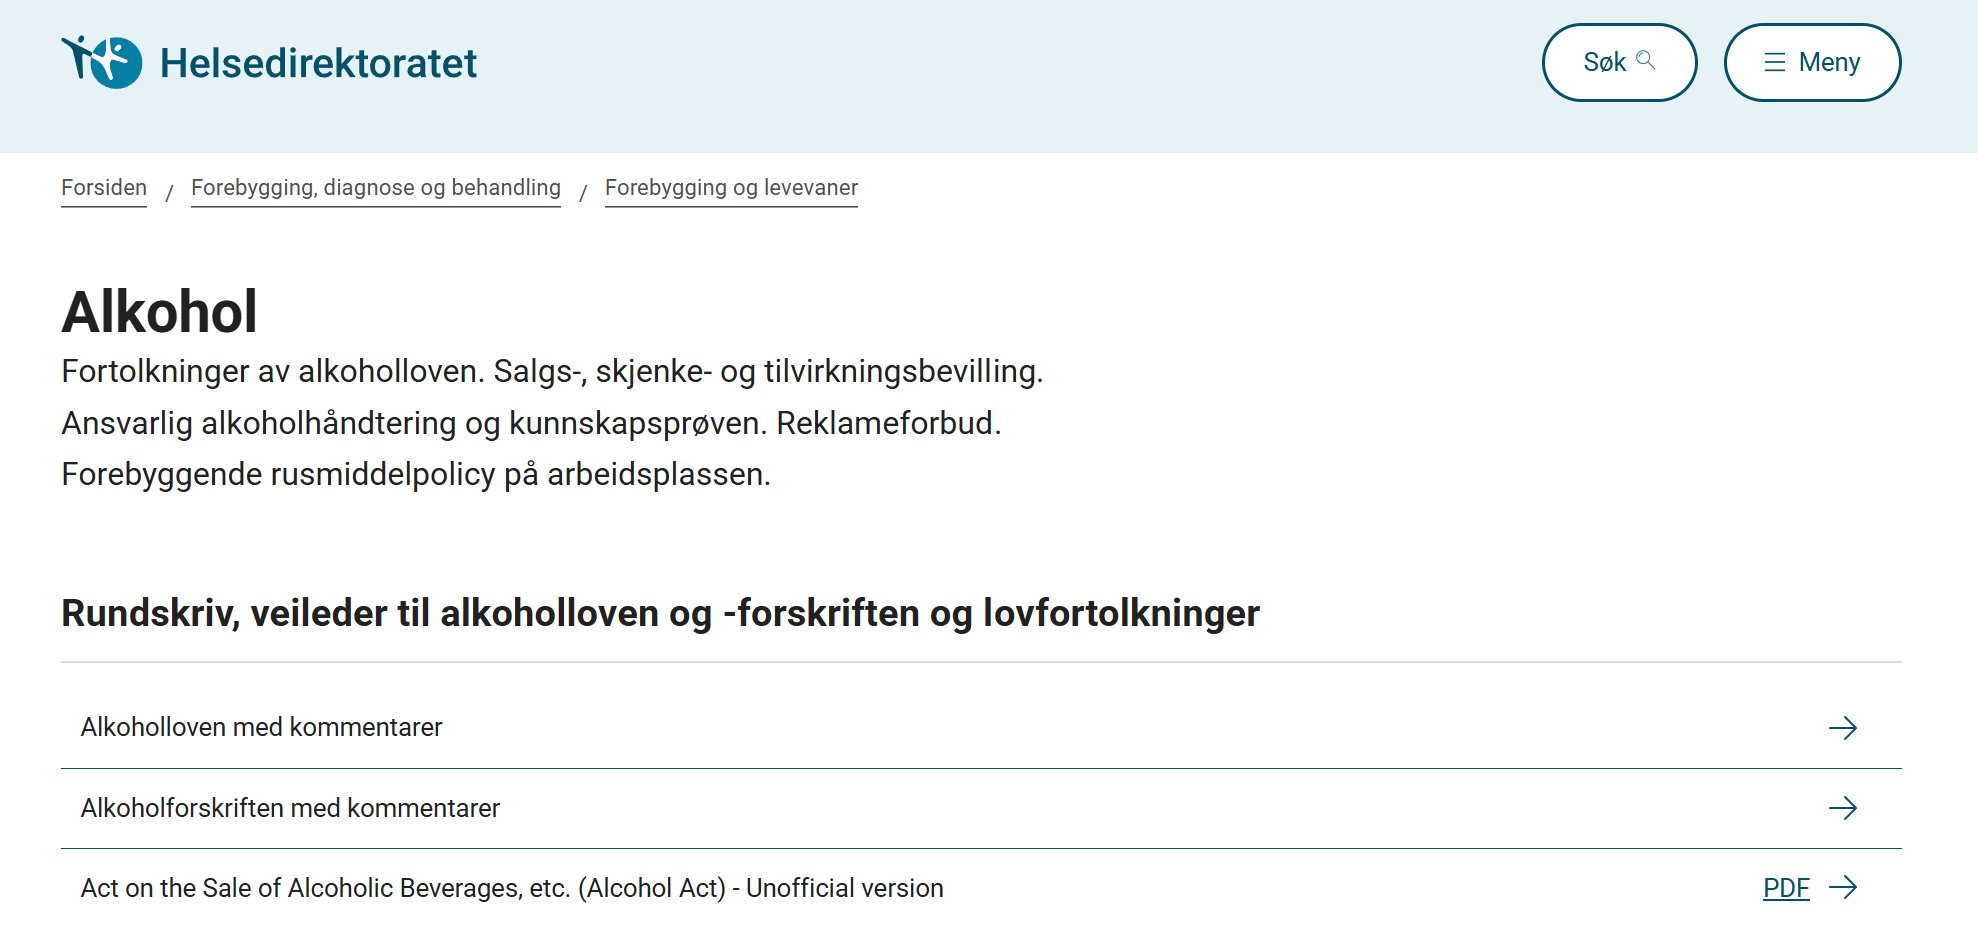
\includegraphics[width=\textwidth]{Images/Figures/Breadcrumbs helsedirektoratet.no.png}
    \caption{Breadcrumbs på helsedirektoratet.no i dag på en temaside}
    \label{fig:hd-breadcrumb-idag}
\end{figure}


\begin{figure}[H]
    \centering
    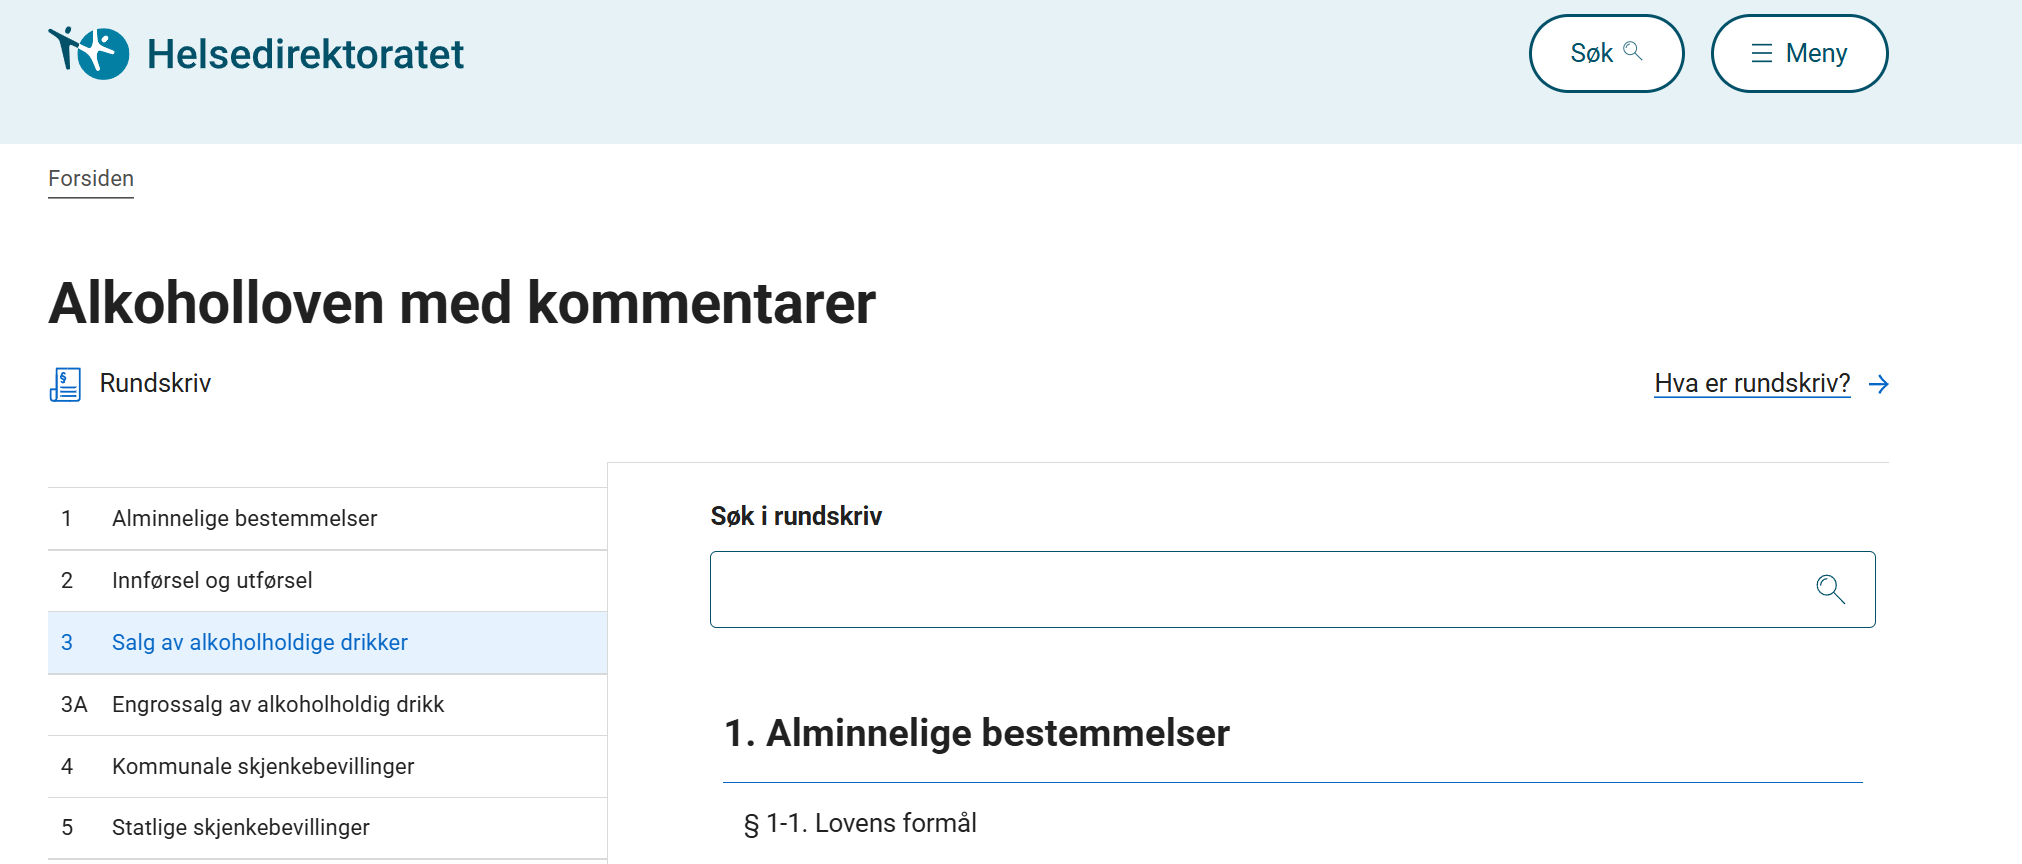
\includegraphics[width=\textwidth]{Images/Figures/Breadcrumbs-side2.png}
    \caption{Breadcrumbs på helsedirektoratet.no i dag på en underside av temasiden}
    \label{fig:hd-breadcrumb-idag-underside}
\end{figure}


% TODO: Legg inn skjermbilde av breadcrumbs på hd.no
% \begin{figure}[H]
%     \centering
%     \includegraphics[width=0.85\textwidth]{Images/Screenshots/hd-breadcrumb-idag}
%     \caption{Brødsmulesti på helsedirektoratet.no -- eksempel fra en
%              retningslinje.}
%     \label{fig:hd-breadcrumb-idag}
% \end{figure}

Breadcrumbsene på helsedirektoratet.no viser stien tilbake til forsiden,
men har noen begrensninger. Breadcrumbsene relfekterer ikke antall klikk og tar med deloverskrifter som man er innom som i figur \ref{fig:hd-breadcrumb-idag} som har med "Forebygging og levevaner", så deretter når du klikker inn til alkoholloven vil breadcrumbsen bli helt kuttet og kun vise til forsiden som vist i figur \ref{fig:hd-breadcrumb-idag-underside}. Hvis man f.eks skulle søkt og klikt seg inn her ville man ikke vist hvor man var i hierarkiet.... 
\subsubsection{Vår løsning}
\label{sec:brodsmulesti-var}

% TODO: Legg inn skjermbilde av vår breadcrumb-komponent
% \begin{figure}[H]
%     \centering
%     \includegraphics[width=0.85\textwidth]{Images/Screenshots/var-breadcrumb}
%     \caption{Brødsmulesti i prototypen -- med kollapsert midtdel og
%              trunkering av lange titler.}
%     \label{fig:var-breadcrumb}
% \end{figure}

Vi implementerte en \texttt{Breadcrumb}-komponent med tre forbedringer
motivert av brukerfeedback (se \autoref{sec:brukerundersokelser}):

\begin{enumerate}
    \item \textbf{Kollapsbar midtdel.} Når stien inneholder tre eller
          flere klikkbare ledd, kollapses mellomleddet til «\texttt{...}»
          ved første visning. Brukeren kan trykke på ellipsen for å
          ekspandere hele stien. Dette holder stien kompakt uten at
          brukeren mister kontekst.

    \item \textbf{Trunkering av lange titler.} Hvert ledd i stien er
          begrenset til en responsiv maksbredde
          (\texttt{clamp(14rem,\,30vw,\,26rem)}) og avskjæres med «…»
          ved overflyt, med full tittel tilgjengelig i
          \texttt{title}-attributtet ved hover.

    \item \textbf{Tilgjengelighet.} Stien er innpakket i et
          \texttt{<nav aria-label="Brodsmulesti">}-element med en
          semantisk \texttt{<ol>}-liste, noe som gir skjermlesere riktig
          kontekstuell informasjon om navigasjonsstien.
\end{enumerate}

% ─────────────────────────────────────────────────────────────
\subsection{Hierarkisk sidenavigasjon}
\label{sec:sidenavigasjon}

\subsubsection{Dagens løsning}
\label{sec:sidenavigasjon-idag}

% TODO: Legg inn skjermbilde av hd.no uten sidebar på retningslinje-side
% \begin{figure}[H]
%     \centering
%     \includegraphics[width=0.85\textwidth]{Images/Screenshots/hd-ingen-sidebar}
%     \caption{Retningslinje-side på helsedirektoratet.no -- ingen lokal
%              innholdsfortegnelse i sidemeny.}
%     \label{fig:hd-ingen-sidebar}
% \end{figure}

Retningslinjer og veiledere på helsedirektoratet.no er lange dokumenter
som gjerne er inndelt i kapitler og underpunkter. Siden mangler en
dedikert sidemeny med innholdsfortegnelse: brukeren navigerer ved å
scrolle eller bruke ankerlenker der de finnes. For fagpersoner som jobber
med komplekse retningslinjer ble dette identifisert som en kilde til
friksjon i brukerundersøkelsene (se \autoref{sec:brukerundersokelser}).

\subsubsection{Vår løsning}
\label{sec:sidenavigasjon-var}

% TODO: Legg inn skjermbilde av SidebarTree i prototypen
% \begin{figure}[H]
%     \centering
%     \includegraphics[width=0.85\textwidth]{Images/Screenshots/var-sidebar}
%     \caption{Hierarkisk sidemeny i prototypen -- ekspanderbart tre med
%              kapittelnummer og aktiv-markering.}
%     \label{fig:var-sidebar}
% \end{figure}

For innholdssider med underdokumenter (f.eks.\ retningslinjer og
veiledere) implementerte vi en \texttt{SidebarTree}-komponent som gir
brukeren en persistent hierarkisk innholdsfortegnelse til venstre for
innholdet. Komponenten har følgende egenskaper:

\begin{itemize}
    \item \textbf{Ekspanderbart tre.} Noder med underdokumenter vises med
          en chevron-indikator og kan ekspanderes og kollapses enkeltvis.
          Allerede besøkte stier holdes ekspandert slik at brukeren
          beholder sin posisjon i dokumenthierarkiet.

    \item \textbf{Aktiv-markering og sti-uthevning.} Gjeldende side
          markeres med fet skrift og primærfargen (\texttt{\#025169}).
          Foreldrenoder i stien utheves med medium skriftvekt, slik at
          brukeren alltid ser sin posisjon i dokumenthierarkiet.

    \item \textbf{Kapittelnummerering.} Hvert ledd viser kapittelnummer
          fra innholdsdokumentet, noe som gjør det enkelt å referere til
          spesifikke deler.

    \item \textbf{Lasteplassholdere.} Mens underdokumenter hentes fra
          API-et, vises en animert spinner per node. Ved feil vises et
          varselikon med forklarende tooltip.
\end{itemize}

% ─────────────────────────────────────────────────────────────
\subsection{Temakort og kategorioversikt}
\label{sec:temakort}

\subsubsection{Dagens løsning}
\label{sec:temakort-idag}

% TODO: Legg inn skjermbilde av kategorinavigasjon på hd.no
% \begin{figure}[H]
%     \centering
%     \includegraphics[width=0.85\textwidth]{Images/Screenshots/hd-kategori-idag}
%     \caption{Kategorinavigasjon på helsedirektoratet.no.}
%     \label{fig:hd-kategori-idag}
% \end{figure}

Helsedirektoratet.no presenterer fagområdene som tekstlenker i en flat
liste. Det er lite visuell differensiering mellom kategoriene, og det er
krevende å få en rask oversikt over hva hvert fagområde inneholder.

\subsubsection{Vår løsning}
\label{sec:temakort-var}

% TODO: Legg inn skjermbilde av CategoryButtons / temaside-forside
% \begin{figure}[H]
%     \centering
%     \includegraphics[width=0.85\textwidth]{Images/Screenshots/var-temakort}
%     \caption{Temakort på forsiden i prototypen -- rutenett med ikon,
%              tittel og hover-effekt.}
%     \label{fig:var-temakort}
% \end{figure}

Forsiden presenterer de syv fagkategoriene som visuelle kort i et
responsivt rutenett (én kolonne på mobil, to på nettbrett, tre på
desktop). Hvert kort inneholder et ikon representativt for fagområdet
og kategoritittelen. En pil animeres inn ved hover og gir visuell
bekreftelse på at kortet er klikkbart. Kortet løfter seg svakt og får
økt skygge ved hover.

Fra et temakort navigerer brukeren til en \textit{temaside hub} som
samler alt innhold innenfor fagområdet, og videre til individuelle
temasider (\textit{temaside leaf}). Denne tostegs-strukturen reduserer
kognitiv last sammenlignet med en flat listestruktur, og gjenspeiler
informasjonsarkitekturen i \autoref{fig:sidehierarki}.

% ─────────────────────────────────────────────────────────────
\subsection{Søkegrensesnitt og kategorifaner}
\label{sec:sokegrensesnitt}

\subsubsection{Dagens løsning}
\label{sec:sokegrensesnitt-idag}

% TODO: Legg inn skjermbilde av søk på hd.no
% \begin{figure}[H]
%     \centering
%     \includegraphics[width=0.85\textwidth]{Images/Screenshots/hd-sok-idag}
%     \caption{Søkeresultater på helsedirektoratet.no.}
%     \label{fig:hd-sok-idag}
% \end{figure}

Søkeresultater på helsedirektoratet.no presenteres som en flat liste
uten kategorisering etter innholdstype. Det er ikke mulig å filtrere
resultatene på fagområde eller innholdstype direkte fra søkesiden, noe
som gjør det krevende å orientere seg i mange treff.

\subsubsection{Vår løsning}
\label{sec:sokegrensesnitt-var}

% TODO: Legg inn skjermbilde av SearchCategoryTabs
% \begin{figure}[H]
%     \centering
%     \includegraphics[width=0.85\textwidth]{Images/Screenshots/var-soketabs}
%     \caption{Kategorifaner i søkeresultatvisningen -- med animert
%              indikatorlinje og antall treff per kategori.}
%     \label{fig:var-soketabs}
% \end{figure}

Søkeresultatene er organisert med en \texttt{SearchCategoryTabs}-komponent
som gir brukeren umiddelbar oversikt over trefffordeling på tvers av
innholdstyper:

\begin{itemize}
    \item \textbf{Faner per innholdstype.} Tabulator-raden viser én fane
          per innholdstype med antall treff, samt en «Alle»-fane. Brukeren
          kan filtrere uten å avbryte søkeflyten.

    \item \textbf{Animert indikatorlinje.} En \texttt{2\,px}-linje under
          aktiv fane animeres horisontalt med \texttt{150\,ms
          ease}-overgang ved faneskifte, noe som gir visuell kontinuitet.

    \item \textbf{Antall treff.} Hvert fane-ledd viser antall treff i den
          respektive kategorien, slik at brukeren raskt kan vurdere om det
          er verdt å filtrere ned.
\end{itemize}

Dette er i tråd med funn fra brukerundersøkelsene
(se \autoref{sec:brukerundersokelser}) om at fagpersoner ønsker å skille
mellom innholdstyper (f.eks.\ retningslinjer vs.\ nyheter) allerede i
søkefasen.

% ─────────────────────────────────────────────────────────────
\subsection{Søkefelt med autofullføring}
\label{sec:autofullføring}

\subsubsection{Dagens løsning}
\label{sec:autofullføring-idag}

% TODO: Legg inn skjermbilde av søkefeltet på hd.no
% \begin{figure}[H]
%     \centering
%     \includegraphics[width=0.85\textwidth]{Images/Screenshots/hd-sokefelt-idag}
%     \caption{Søkefelt på helsedirektoratet.no -- ingen autofullføring.}
%     \label{fig:hd-sokefelt-idag}
% \end{figure}

Søkefeltet på helsedirektoratet.no tilbyr ikke autofullføring eller
sanntidsforslag mens brukeren skriver. Brukeren må fullføre søkeordet
manuelt og trykke Enter for å se resultater. Det finnes heller ingen
tastaturnavigasjon i en forslagsliste, noe som øker antall klikk som
kreves for å nå riktig innhold.

\subsubsection{Vår løsning}
\label{sec:autofullføring-var}

% TODO: Legg inn skjermbilde av SearchForm med åpen forslagsliste
% \begin{figure}[H]
%     \centering
%     \includegraphics[width=0.85\textwidth]{Images/Screenshots/var-autofullføring}
%     \caption{Søkefelt i prototypen med autofullføring -- uthevet match og
%              aktiv markering ved tastaturnavigasjon.}
%     \label{fig:var-autofullføring}
% \end{figure}

Vi implementerte en \texttt{SearchForm}-komponent med en integrert
\texttt{SearchSuggestions}-rullegardin som gir brukeren umiddelbar
tilbakemelding under skriving:

\begin{itemize}
    \item \textbf{Sanntidsforslag.} Komponenten henter forslag fra
          backend via \texttt{useSearchSuggestionsQuery()} mens
          brukeren skriver. Hvert forslag viser tittel og
          innholdstypeetikett.

    \item \textbf{Uthevede treff.} Den delen av forslaget som matcher
          søkestrengen fremheves med fet skrift i primærfargen
          \texttt{\#025169}, slik at brukeren raskt ser relevansen.

    \item \textbf{Tastaturnavigasjon.} Brukeren kan navigere i
          forslagslisten med piltast opp/ned, velge med Enter og lukke
          listen med Escape -- uten å forlate tastaturet.

    \item \textbf{Tilgjengelighet.} Søkefeltet er merket med ARIA-rolle
          \texttt{combobox} og forslagslisten med \texttt{listbox},
          i tråd med WAI-ARIA-mønsteret for autofullføring.
\end{itemize}

% ─────────────────────────────────────────────────────────────
\subsection{Barngruppe-rullegardin i søkeresultater}
\label{sec:barngruppe}

\subsubsection{Dagens løsning}
\label{sec:barngruppe-idag}

% TODO: Legg inn skjermbilde av søkeresultat for temaside på hd.no
% \begin{figure}[H]
%     \centering
%     \includegraphics[width=0.85\textwidth]{Images/Screenshots/hd-temasideresultat-idag}
%     \caption{Søkeresultat for en temaside på helsedirektoratet.no --
%              ingen underinnhold synlig.}
%     \label{fig:hd-temasideresultat-idag}
% \end{figure}

Søkeresultater for temasider på helsedirektoratet.no vises som enkle
lenker uten innsikt i hva slags underinnhold temasiden inneholder.
Brukeren må navigere inn på siden for å finne ut om den er relevant,
noe som øker antall klikk i søkeflyten.

\subsubsection{Vår løsning}
\label{sec:barngruppe-var}

% TODO: Legg inn skjermbilde av ChildGroupDropdown i søkeresultat
% \begin{figure}[H]
%     \centering
%     \includegraphics[width=0.85\textwidth]{Images/Screenshots/var-barngruppe}
%     \caption{Barngruppe-rullegardin i søkeresultatkort -- sidestilt
%              liste over underinnhold med automatisk viewport-tilpasning.}
%     \label{fig:var-barngruppe}
% \end{figure}

Søkeresultatkort for temasider med underinnhold viser en
\texttt{ChildGroupDropdown}-komponent som gjør det mulig å forhåndsvise
innholdet uten å forlate søkesiden:

\begin{itemize}
    \item \textbf{Hover og lås.} Rullegardinmenyen aktiveres ved hover
          over en undergruppe og kan låses åpen med klikk, slik at
          brukeren kan sammenligne grupper uten at lista lukkes.

    \item \textbf{Sidestilt posisjonering.} Listen posisjoneres til
          høyre for gruppen (\texttt{left-full ml-2}) for å unngå at
          den dekker søkelisten bak.

    \item \textbf{Automatisk viewport-tilpasning.} Dersom listen vil
          gå utenfor skjermens nederkant, flipper komponenten listen
          oppover via \texttt{useLayoutEffect}, slik at innholdet
          alltid er synlig.

    \item \textbf{Forsinkelse ved utgang.} Muspekeren kan flyttes fra
          gruppe til liste uten at lista lukkes, takket være en
          \texttt{150\,ms} forsinkelse ved museutgang.
\end{itemize}

% ─────────────────────────────────────────────────────────────
\subsection{Kapittelpaginering i hierarkisk innhold}
\label{sec:kapittelpaginering}

\subsubsection{Dagens løsning}
\label{sec:kapittelpaginering-idag}

% TODO: Legg inn skjermbilde av bunnen av en retningslinje på hd.no
% \begin{figure}[H]
%     \centering
%     \includegraphics[width=0.85\textwidth]{Images/Screenshots/hd-ingen-paginering}
%     \caption{Bunn av en retningslinje på helsedirektoratet.no --
%              ingen forrige/neste-navigasjon.}
%     \label{fig:hd-ingen-paginering}
% \end{figure}

Retningslinjer og veiledere på helsedirektoratet.no tilbyr ingen
sekvensiell navigasjon mellom kapitler. For å gå til neste kapittel
må brukeren enten scrolle tilbake til innholdsfortegnelsen, bruke
sidemenylenker der disse finnes, eller huske kapittelnummer selv.
Dette skaper friksjon i lineær gjennomlesning av lange dokumenter.

\subsubsection{Vår løsning}
\label{sec:kapittelpaginering-var}

% TODO: Legg inn skjermbilde av forrige/neste-navigasjon i prototypen
% \begin{figure}[H]
%     \centering
%     \includegraphics[width=0.85\textwidth]{Images/Screenshots/var-kapittelpaginering}
%     \caption{Kapittelpaginering i prototypen -- stilede forrige/neste-knapper
%              med kapittelnummer og tittel.}
%     \label{fig:var-kapittelpaginering}
% \end{figure}

Nederst på hver innholdsside implementerte vi en
kapittelpagineringslinje som gir brukeren et tydelig veipunkt mellom
kapitler:

\begin{itemize}
    \item \textbf{Forrige og neste.} Navigasjonsraden viser knapper
          for forrige og neste kapittel med kapittelnummer og tittel
          trunkert til én linje, slik at brukeren vet hva som venter
          uten å navigere dit.

    \item \textbf{Visuell retningsindikator.} Venstre- og høyrepil
          i en avrundet sirkel med primærfarge (\texttt{\#025169})
          skiller tydelig retning på navigasjonen.

    \item \textbf{Bakgrunnsprehenting.} Forrige og neste side hentes
          fra API-et i bakgrunnen ved sideinnlasting, slik at
          navigasjonen oppleves umiddelbar.

    \item \textbf{Konsistens med sidemeny.} Kapittelnummer og tittel
          i pagineringen samsvarer med visningen i
          \texttt{SidebarTree}-menyen, noe som forsterker
          plasseringsfølelsen i dokumenthierarkiet.
\end{itemize}



% ─────────────────────────────────────────────────────────────
\subsection{Universell utforming og brukervennlighet}
\label{sec:nav-wcag}

\subsubsection{navigasjonskomponentene}

Offentlige nettjenester er lovpålagt å følge WCAG~2.1~AA (se
\autoref{sec:wcag-teori}). Helsedirektoratets tilgjengelighetserklæring
erklærer delvis samsvar og peker på konkrete mangler i tastaturnavigasjon
og ARIA-merking av interaktive elementer \cite{uustatus-helsedir}.
Navigasjonskomponentene i prototypen adresserer disse punktene direkte.

\paragraph{Hopplenke --- kriterium 2.4.1}
Hopplenken er første fokuserbare element på siden og lar tastaturbrukere
hoppe over gjentakende header og meny. Vi bruker \texttt{SkipLink} fra
Digdir Designsystemet, den norske offentlige sektorens felles
komponentbibliotek:

\begin{minted}[fontsize=\small, frame=lines]{jsx}
// AppLayout.tsx
<SkipLink href="#main-content">Hopp til hovedinnhold</SkipLink>
<AppHeader ... />
<main id="main-content">
  <Outlet />
</main>
\end{minted}

\paragraph{WAI-ARIA combobox-mønster i søkefelt --- kriterium 4.1.2}
Helsedirektoratets søkefelt har ingen ARIA-merking. \texttt{SearchForm}
i prototypen implementerer det fulle WAI-ARIA \textit{combobox}-mønsteret
slik at skjermlesere korrekt formidler søkefeltets tilstand og aktiv
markering i forslagslisten. Forslagslisten støtter i tillegg fullstendig
tastaturnavigasjon (kriterium 2.1.1):

\begin{minted}[fontsize=\small, frame=lines]{jsx}
// SearchForm.tsx
<input
  role="combobox"
  aria-expanded={showSuggestions && suggestions.length > 0}
  aria-controls={listboxId}
  aria-activedescendant={
    activeIndex >= 0 ? `${listboxId}-option-${activeIndex}` : undefined
  }
  aria-autocomplete="list"
  aria-label="Søk"
  onKeyDown={handleKeyDown}  // ArrowDown/Up, Enter, Escape
/>
\end{minted}

\paragraph{Semantisk navigasjonsmarkering --- kriterium 4.1.2, 2.4.6}
Alle navigasjonsregioner bruker \texttt{<nav>} med beskrivende
\texttt{aria-label}, slik at skjermlesere kan tilby hurtignavigasjon
mellom landmark-regioner. Aktiv side markeres programmatisk med
\texttt{aria-current}, og knapper for kapittelpaginering har eksplisitt
\texttt{aria-label} med kapittelnummer:

\begin{minted}[fontsize=\small, frame=lines]{jsx}
// SidebarTree.tsx
<nav aria-label="Innholdssider">
  <button aria-current={isOverviewActive ? "page" : undefined}>
    Oversikt
  </button>
</nav>

// PageContent.tsx
<nav aria-label="Navigasjon mellom kapitler">
  <button aria-label={`Gå til forrige kapittel ${previousPage.numbering}`}>
    ...
  </button>
  <button aria-label={`Gå til neste kapittel ${nextPage.numbering}`}>
    ...
  </button>
</nav>
\end{minted}

Dekorative ikoner og skilletegn er konsekvent merket med
\texttt{aria-hidden="true"} for å skjules fra skjermlesere (kriterium
1.1.1), og primærfargen \texttt{\#025169} fra Digdir Designsystemet
overstiger AA-kravet på 4,5:1 i fargekontrast mot hvit bakgrunn
(kriterium 1.4.3).

\subsubsection{På tvers av enheter}
Ved bruk av nettsiden på mobilen er det lagt til rette for bedre utforming